%
% Template file for software architecture design description in the
% DIKU course Software Architecture and Software Design. Please do
% not distribute outside the course
%
% Based on a template (c) by Woods and Rozanski (2011) available at
%
%    http://www.viewpoints-and-perspectives.info
%
% Instructions:
%
% 1) change the metadata commands below (\groupname) etc. to fit your
%     project
% 2) uncomment the overwriting of the \instructions command to remove
%     instructions
% 3) write your architectural description...
%
% Contact: klausmh@di.ku.dk
%
\documentclass[a4paper,11pt]{report}
\usepackage{natbib}
\usepackage[pdftex]{graphicx}
\usepackage{color}
\usepackage[table]{xcolor}
\usepackage{hyperref}
\usepackage{lastpage}
\usepackage{longtable}

% Meta-data for report
\newcommand{\systemname}{Online Rental System}
\newcommand{\groupname}{Group $\Omega$}
\newcommand{\contactdetails}{Henrik Bendt: gwk553@ku.dk\\Nicolai Willems ntb459@ku.dk\\Søren Egede Pilgård: vpb984@ku.dk}

% Typesetting of instructions for using the template,
% remove by renewing command
\newcommand{\instructions}[1]{
  \noindent\colorbox{lightgray}{%
    \parbox{\linewidth}{%
      #1
    }%
  }%
 \vspace{0.1cm}
}
% \renewcommand{\instructions}[1]{} % Uncomment to remove instructions

% We use the below command for figure captions since
% the figure environment does not play nicely with
% \colorbox. The "real" way to create figures is like this:
%   \begin{figure}[ht!]
%     \centering
%     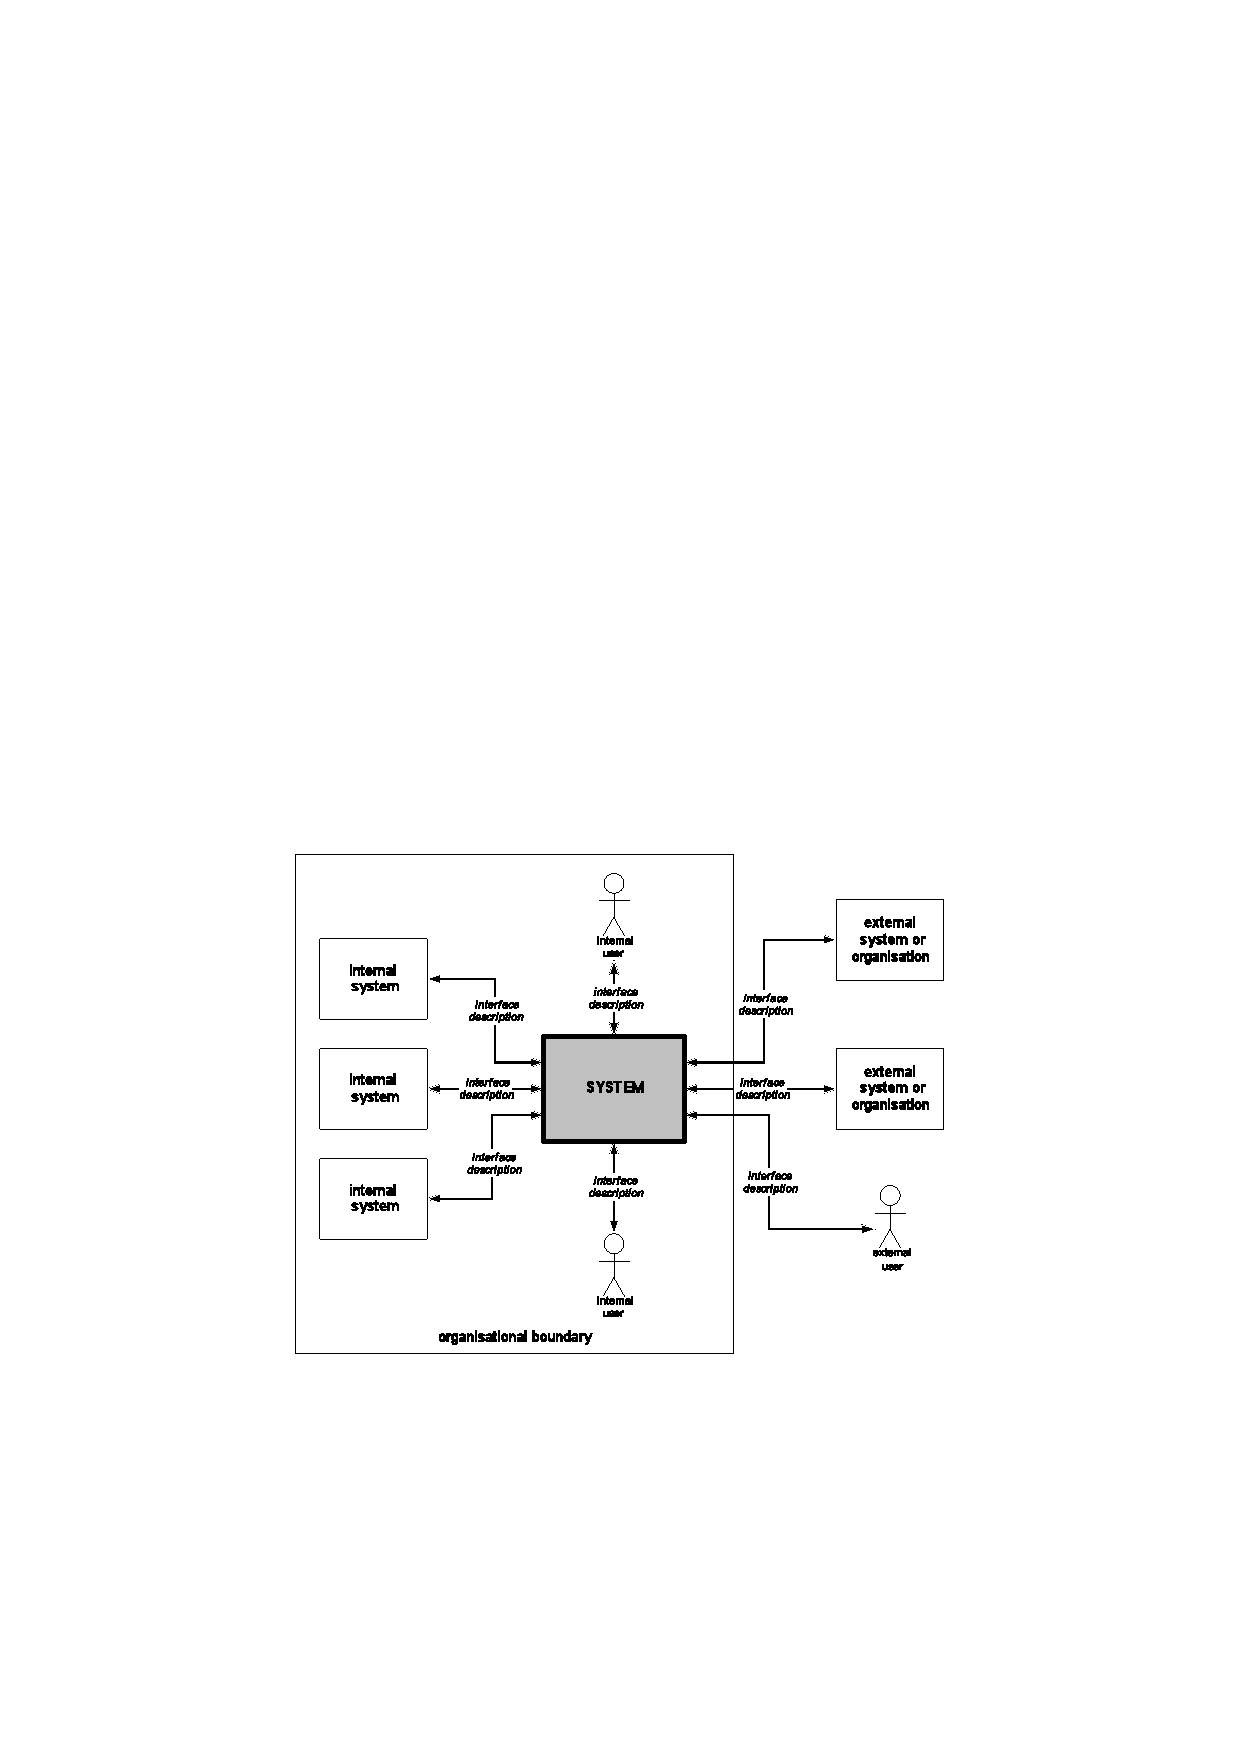
\includegraphics[width=0.8\textwidth]{figures/systemcontext}
%    \caption{System context}
%     \label{fig:systemcontext}
%   \end{figure}
\newcommand{\mycaption}[1]{
  \addtocounter{figures}{1}
  Figure \arabic{figures}. #1
}

\setlength\parskip{1em}
\setlength\parindent{0em}

% Change font family to Helvetica
\renewcommand{\rmdefault}{phv}
\renewcommand{\sfdefault}{phv}

% Set headers and footers
\usepackage{fancyhdr}
\pagestyle{fancy}
\fancyhf{}
\fancyhead[C]{Software Architecture of \systemname\ }
\fancyfoot[C]{\footnotesize Page \thepage\ of \pageref{LastPage}}


% Added commands for good stuff
\newcommand{\seller}{ seller }
\newcommand{\buyer}{ buyer }

\begin{document}
%
% Title page
%
\newcommand{\HRule}{\rule{\linewidth}{0.5mm}}
\begin{titlepage}

  \begin{center}

    % Title
    \vspace*{4cm}
    \HRule \\[0.4cm]
    { \huge \bfseries \systemname}\\[0.4cm]
    \HRule \\[1.5cm]

    {\Large Software Architecture Description}

    \vfill
  \end{center}

  % Author, version, date
  \begin{flushleft}
    {\LARGE \groupname}\\[0.2cm]
    {\large \contactdetails}\\[0.2cm]
   {\large \today}
  \end{flushleft}
\end{titlepage}

%
% Version table
%
\newpage
\chapter*{Version history}

\begin{center}
  \begin{tabular}[h!]{| l | l | l | p{8 cm} |}
    \hline
    \rowcolor{gray}
    Version & Date & Author & Comments \\
    \hline
    \hline
    1 & 2014-09-03 & HB & Filling out ch 1 and 5.1\\
    \hline
    2 & 2014-09-08 & NW & Adding figure and group name \\
    \hline
  \end{tabular}
\end{center}

%
% Table of contents
%
\setcounter{tocdepth}{1}
\tableofcontents

%
% Main text
%
\chapter{Introduction}
\label{cha:introduction}
\thispagestyle{fancy}

In this report we define a person who rent out items as a \textit{seller} and a person who rent items as a \textit{buyer}. We shall try to be consistent with this convention.

\section{Purpose and scope}
\label{sec:purpose-scope}
The project is about developing an online renting system (as a website), from
here on referred to as ORS. In the system it should be possible for users to
rent out items to other users for a small fee (possibly none) and a safety
deposit (in case of return of damaged items). When a user wants to rent a
provided item, the system should provide the contact information to the
providing user. The business case is to take a small percentage or amount from
the rental fee when providing the contact information.

Users should be able to search for specific items or item categories,
geographical locations, price ranges, etc. They should also be able to queue up
for a specific provided item (by another user) if it is already rented out or
multiple other people are interested in renting the item.

It should be possible to share what you are renting out on Facebook or Twitter.

A scenario could be a person, owning an electric saw, which he is not using, but
don't want to sell. He could then be interested in making some money off this
item, by renting it to people in his area (for example his home city Copenhagen,
or maybe in all of Sjælland, etc.). Instead of setting up fliers in his local
area (like in the local grocery store, local sports center, etc.) he puts the
item up on ORS because it is easy and fast. Now, people in need of such electric
saw contacts him without him doing anything but making the electric saw
available for renters.

The system is to be deployed and runned on a cloud system like Amazon Cloud. It should use an external paying system like Paypal.

\subsection{Scope}
\paragraph{Included}
\begin{itemize}
\item Supply items for rent
\item Search for items for rent
\item Requests items for rent
\item Billing + Deposits when renting
\item Tracking of items rented out (which user, living where)
\item Website handling the above
\end{itemize}

\paragraph{Excluded}
\begin{itemize}
\item Sales
\item Errors + Damage to items -- handling these cases
\item Hardware for the server -- we shall use a cloud solution.
\item Verification of transfers (how to verify an item is physically rented/given to a user and returned again).
\end{itemize}

\section{Audience}
\label{sec:audience}
The primary purpose of this document is communication between system architects
and system developers designing and building the actual system.
Further it can be used by sponsors and other stakeholders to get an overview of
the system.

\section{Status}
\label{sec:status}
The system is currently undergoing architectual design, as we are developing
the goals and ideas behind the system.

Our future plans include developing an architectual prototype, that shall show
your intentions and what external/internal components are required.

\section{Architectural design approach}
\label{sec:arch-design-appr}


\chapter{Glossary}
\label{cha:glossary}
\thispagestyle{fancy}

\chapter{System stakeholders and requirements}
\label{cha:syst-stak-requ}
\thispagestyle{fancy}

\section{Stakeholders}
\label{sec:stakeholders}
Here are the stakeholders, their interest and concerns about the system and whom their role is fulfilled by in ORS.
%\begin{table}[H]
\begin{center}
    \begin{longtable}[H]{| l |  p{6cm} | p{2cm} |}
    \hline
    \textbf{Stakeholder} & \textbf{Interest, needs and concerns} & \textbf{Held
        by} \\
    \hline
    Architect & Interested in the success of the system and is very concerned
        with the design and development. He is also concerned about the project 
        fulfilling the found/given requirements. He needs a requirement
        specification and requires an assisting organization to carry
        out/develop the designed system. & ORS \\
    \hline
    Users &  Interested in a well-functioning and highly available product,
        with high standards on security in transactions of items. Their needs
        are based on the idea that they either provide items or would like to
        ``rent'' an item. They are primarily concerned with their personal
        security and the well-being of the rented item in question & Everyone \\
    \hline
    Acquirers & Interested in a successful and relative quick launch of the system along with the business model of the system and eventual marketing and advertising. & Possible investors, ORS owners \\
    \hline
    Assessors & Interested mainly around the legality and validity of the
        protocols surrounding the system. Their needs are in the area of
        transparency and documentation of the system, such that the are able to
        assess the system. & Lawyers and ORS Legal team, maybe external
        accountants\\
    \hline
    Communicators & Interested in the creation of the license agreements and rental contracts for the site. & Lawyers and ORS Legal team\\
    \hline
    Developers & Interested in the design of the software system and is concerned with the modularity (that the system is easy to maintain/expand) and performance. & ORS Development team\\
    \hline
    Maintainers & Interested in the modularity of the system, defining how easy the system is to fix and expand, along with the platform (here Amazon Cloud) the system is to be runned on. & ORS Admins \\
    \hline
    Production Engineers & Interested in the different parts of the system (including external systems like Paypal), the ease of deployment of the system and the platform it runs on. & Amazon and ORS Admins\\
    \hline
    Suppliers & Interested in the use and integration of their external systems (for example the billing system of Paypal and the Amazon cloud). & Paypal, Amazon\\
    \hline
    Support Staff & Interested in the functionality and stability of the system, along with the usability; how easy it is to administrate users and to use the site. & ORS Admins \\
    \hline
    System Administrators & Interested in the stability and accessibility to the system (when using Amazon cloud, what kind of access do we have to it and how much control do we have) and the platform/hardware it is runned on, giving and idea of how easy it is to fix eventual problems, with respect to both software and hardware. & ORS Admins and Amazon \\
    \hline
    Testers & Interested in early access to the system along with the stability and functionality of the system, which they test. & Possible early users\\
    \hline
  \end{longtable}
\end{center}
%\end{table}


\section{Overview of requirements}\label{sec:overv-requ}
\begin{center}
  \begin{tabular}[h]{| l |  l |}
    \hline
    \textbf{Reference} & \textbf{Requirement description} \\
    \hline
    R1 & User creating an item to rent out (usability)\\
    \hline
    R2 & User finding and renting item (usability)\\
    \hline
    R3 & Admin removing item from site (usability)\\
    \hline
    R4 & Many users try to rent same item (usability, accessibility)\\
    \hline
    Q1 & A user tries to access an item under heavy load (performance, availability)\\
    \hline
    Q2 & A user tries to access the site without valid credentials (security)\\
    \hline
    Q3 & A user rents an item under normal load (performance, security)\\
    \hline
  \end{tabular}
\end{center}

\section{System scenarios}
\label{sec:system-scenarios}
The following two sections tries to describe scenarios related to the above
requirements. Their role is to dig into the requirements, and make them more
``alive''.

\subsection{Functional scenarios}
\label{sec:functional-scenarios}
The scenarios concerning the functionality of the system are listed and
described below. The template is the one from \cite{rozanski2011software}
chapter 10.

\begin{description}
    \item[Overview] R1 - A user creating an item in the system
    \item[System state] The user is authenticated and logged in
    \item[System environment] The environment has no issues
    \item[External stimulus] The user submits a request to add an item for rent
        in the database
    \item[Required system response] The system shall start processing the
        incoming record and tell the user, that their item will be added
        shortly.
\end{description}

\begin{description}
    \item[Overview] R2 - The user finds and rents an item
    \item[System state] The system contains at least one item, that is
        available for renting out.
    \item[System environment] The system is in its normal environment, and the
        person renting out, is ready to deliver.
    \item[External stimulus] The user request the system to facilitate a
        ``rent''
    \item[Required system response] The system shall notify the person renting
        out about interest, afterwards it shall notify the interested party on
        the availability of the requested item.
\end{description}


\subsection{System quality scenarios}
\label{sec:syst-qual-scen}
This section closely mimics the previous, but concerns the quality scenarios
instead.

\begin{description}
    \item[Overview] Q1 - A user tries to access an item while the system is
        under heavy load.
    \item[System state] The system is in its normal working condition, with at
        least one user signed up
    \item[System environment] The system is working correctly and has 10.000
        active users pr minute
    \item[Environment change] A spike in traffic, at around 100.000 users pr
        minute, accessing the system.
    \item[Required system behavior] The system is expected to scale within the
        first 10 seconds, and return error pages to less than 10.000 users.
\end{description}

\begin{description}
    \item[Overview] Q3 - A user rents an item under normal load
    \item[System state] The system has at least two users has signed up, one
        renting out another renting.
    \item[System environment] The system is handling its average 10.000 users pr
        minute, the system' environment is functioning normally.
    \item[Environment change] A user asks to rent an item
    \item[Required system behavior] The system is expected to respond to
        incoming requests in less than 0.1 second
\end{description}


\chapter{Architectural forces}
\label{cha:architectural-forces}
\thispagestyle{fancy}

\section{Goals}
\label{sec:goals}
We have the following functional and non-functional goals.

\textbf{Functional goals:}
\begin{description}
  \item[satG1] A user shall be able to rent an item.
  \item[satG2] A user shall be able to rent out an item.
  \item[satG3] The system shall be able to recieve payments and forward payments.
  \item[infG1] A user shall be informed about the availability of a given item within 24 hours.
  \item[infG2] A user shall be able to view evaluations of items.
\end{description}
where satG is ``satisfaction goal'' and infG is ``information goal''.

\textbf{Non-functional goals:}
\begin{description}
  \item[devG1] We shall seek to reuse as many components already available as possible, to limit the development time as much as possible.
  \item[qosG1] We shall seek to maintain the uptime of the site as high as possible.
  \item[qosG2] The system shall keep personal information (like name, address, etc.) secure.
  \item[qosG3] The system shall keep personal information apart from the items. %TODO add explanation
  \item[qosG4] The system shall not handle payment information --  this should be handled by an external party.
  \item[arcG1] We shall determine the role of the system in relation to the seller and the buyer.
\end{description}
where devG is ``development goal'', qosG is ``quality of service goal'' and arcG is ``architectural constraints goal''.


\section{Constraints}
\label{sec:constraints}
We have the following constraints
\begin{itemize}
  \item The system employs client-server model.
  \item The system employs $n$-layer architecture (e.g. a front-end, an application server, a database server, etc.).
  \item The front-end GUI of the system is written in HTML and corresponding technologies.
  \item The system must be independent from hardware specifications, as we do not know what it will run on (only that it will be runned on a cloud solution).
  \item All technical interactions in the system and user transactions must be logged.
\end{itemize}


\section{Architectural principles}
\label{sec:arch-princ}
The system shall seek to follow these principles.
\begin{center}
  \begin{tabular}[h!]{| >{\columncolor{gray}}p{0.28\textwidth} | p{0.65\textwidth} |}
    \hline
    Principle reference & P1. Use of open source\\
    \hline
    Principle statement & ORS uses, where possible, only open source components, both externally and internally. \\
    \hline
    Rationale & Open source software is free and thus supports a cheaper solution with no licensing problems. With the limited amount of capital involved in the project, open source adds much functionality for free.\\
    \hline
    Implications & 
      \begin{itemize}
        \item Limited support for the use of open source components -- we do not pay anyone for this support, and are thus dependent on the community of the component.
        \item Extra care must be taken with respect to open source components licenses, as these may be diverse and imply special use of these components.
        \item Extension of open source components is possible (with respect to the given license).
      \end{itemize}\\
    \hline
  \end{tabular}
\end{center}

\begin{center}
  \begin{tabular}[h!]{| >{\columncolor{gray}}p{0.28\textwidth} | p{0.65\textwidth} |}
    \hline
    Principle reference & P2. No payment information storage\\
    \hline
    Principle statement & ORS will not, at any point, handle or store payment information provided by the user. This will be handled by an external component.\\
    \hline
    Rationale & The law about handling payment information is complex and strict and the liability with handling payment information is too great for ORS.\\
    \hline
    Implications & 
      \begin{itemize}
        \item Data cannot be temporarily stored in the system, but must be send directly to the external billing service.
        \item We must use an external billing service and thus conform to this API.
      \end{itemize}\\
    \hline
  \end{tabular}
\end{center}

\begin{center}
  \begin{tabular}[h!]{| >{\columncolor{gray}}p{0.28\textwidth} | p{0.65\textwidth} |}
    \hline
    Principle reference & P3. Usability before functionality\\
    \hline
    Principle statement & ORS will prioritize usability over functionality, which can be used in the development of the system.\\
    \hline
    Rationale & The business cannot run without users, and users will not use a system with lousy usability. Thus the quality of the system is very depended on usability. This principle follows from many modern companies, like Amazon and Apple, who develops around usability and quality before functionality. \\
    \hline
    Implications & 
      \begin{itemize}
        \item Functionality will be added slower.
        \item Newly added functionality should be easily used from deployment, creating direct value for the users instead of confusion and/or frustration.
      \end{itemize}\\
    \hline
  \end{tabular}
\end{center}


\chapter{Architectural views}
\label{cha:architectural-views}
\thispagestyle{fancy}

\section{Context view}
\label{sec:context-view}



\newcounter{figures}
\subsection{Context diagram}
\label{sec:context-diagram}

See figure \ref{fig:context}.

\begin{figure}[h!]
  \centering
  \includegraphics[width=0.7\textwidth]{figures/context_drawing}
  \caption{The context of the system}
  \label{fig:context}
\end{figure}




\subsection{Interaction scenarios}
\label{sec:inter-scen}
Examples of interaction scenarios:

A user setting up an item.
\begin{itemize}
  \item User creates login to the site, adding personal information like name, address, payment info.
  \item User creates item, a hammer, he wants to rent out, setting renting price and deposit price.
  \item User shares the item via the site on Facebook.
\end{itemize}

A user rents an item.
\begin{itemize}
  \item User creates login to the site, adding personal information like name, address, payment info.
  \item User searches for an item, a hammer.
  \item User finds a hammer he wants to rent in his local area, Copenhagen.
  \item User rents the hammer from user and pays via the system via Paypal.
  \item The user renting out the hammer recieves the payment via Paypal.
\end{itemize}

\section{Functional view}
\label{sec:functional-view}

\begin{figure}
\label{fig:funcView}
%TODO add functional view. This figure is referenced in \ref{sec:functional-elements} for interfaces.
\end{figure}

\subsection{Functional elements}
\label{sec:functional-elements}
These are the functional elements as presented in figure \ref{fig:funcView}.
\begin{center}
  \begin{tabular}[h!]{| >{\columncolor{gray}}p{0.28\textwidth} | p{0.65\textwidth} |}
    \hline
    Element name & Handler\\
    \hline
    Responsibilities &
    \begin{itemize}
      \item Forwards user requests to Application layer
      \item Returns answers as a HTML-page
    \end{itemize}\\
    \hline
    Interfaces -- required & See figure \ref{fig:funcView}\\
    \hline
    Interfaces -- provided & See figure \ref{fig:funcView}\\
   \hline
  \end{tabular}
\end{center}

\begin{center}
  \begin{tabular}[h!]{| >{\columncolor{gray}}p{0.28\textwidth} | p{0.65\textwidth} |}
    \hline
    Element name & Render\\
    \hline
    Responsibilities &
    \begin{itemize}
      \item Returns the HTML for a requested page.
    \end{itemize}\\
    \hline
    Interfaces -- required & See figure \ref{fig:funcView}\\
    \hline
    Interfaces -- provided & See figure \ref{fig:funcView}\\
   \hline
  \end{tabular}
\end{center}

\begin{center}
  \begin{tabular}[h!]{| >{\columncolor{gray}}p{0.28\textwidth} | p{0.65\textwidth} |}
    \hline
    Element name & Action Control\\
    \hline
    Responsibilities &
    \begin{itemize}
      \item Directs user requests
    \end{itemize}\\
    \hline
    Interfaces -- required & See figure \ref{fig:funcView}\\
    \hline
    Interfaces -- provided & See figure \ref{fig:funcView}\\
   \hline
  \end{tabular}
\end{center}

\begin{center}
  \begin{tabular}[h!]{| >{\columncolor{gray}}p{0.28\textwidth} | p{0.65\textwidth} |}
    \hline
    Element name & Query handler\\
    \hline
    Responsibilities &
    \begin{itemize}
      \item Translate requests to queries for
        \begin{itemize} 
          \item Adding item
          \item Removing item
          \item Find item
          \item Queuing to item
        \end{itemize}
    \end{itemize}\\
    \hline
    Interfaces -- required & See figure \ref{fig:funcView}\\
    \hline
    Interfaces -- provided & See figure \ref{fig:funcView}\\
   \hline
  \end{tabular}
\end{center}

\begin{center}
  \begin{tabular}[h!]{| >{\columncolor{gray}}p{0.28\textwidth} | p{0.65\textwidth} |}
    \hline
    Element name & Item Store\\
    \hline
    Responsibilities &
    \begin{itemize}
      \item Interface for the storing and handling of items.
    \end{itemize}\\
    \hline
    Interfaces -- required & See figure \ref{fig:funcView}\\
    \hline
    Interfaces -- provided & See figure \ref{fig:funcView}\\
   \hline
  \end{tabular}
\end{center}

\begin{center}
  \begin{tabular}[h!]{| >{\columncolor{gray}}p{0.28\textwidth} | p{0.65\textwidth} |}
    \hline
    Element name & Transaction\\
    \hline
    Responsibilities &
    \begin{itemize}
      \item Handles transactions for renting out items; seller to buyer
      \item Handles transactions for returning items; buyer to seller
      \item Redirects billing to third party billing service
      \item Asserts items exists
    \end{itemize}\\
    \hline
    Interfaces -- required & See figure \ref{fig:funcView}\\
    \hline
    Interfaces -- provided & See figure \ref{fig:funcView}\\
   \hline
  \end{tabular}
\end{center}

\begin{center}
  \begin{tabular}[h!]{| >{\columncolor{gray}}p{0.28\textwidth} | p{0.65\textwidth} |}
    \hline
    Element name & Event Log\\
    \hline
    Responsibilities &
    \begin{itemize}
      \item Logs transactions between users (renting of an item, returning of an item)
    \end{itemize}\\
    \hline
    Interfaces -- required & See figure \ref{fig:funcView}\\
    \hline
    Interfaces -- provided & See figure \ref{fig:funcView}\\
   \hline
  \end{tabular}
\end{center}


\subsection{Functional scenarios}
\label{sec:functional-scenarios-1}
The two former functional scenarios are here presented in sequence diagrams.

\textbf{R1} - A user creating an item in the system, is presented in figure
\ref{fig:r1-sequence}

\textbf{R2} - The user finds and rents an item, is presented in figure
\ref{fig:r2-sequence}

\begin{figure}[ht]
    \centering
    \caption{The function scenario R1}
    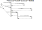
\includegraphics[width=0.8\textwidth]{figures/r1-sequence}
    \label{fig:r1-sequence}
\end{figure}

\begin{figure}[ht]
    \centering
    \caption{The function scenario R2}
    
\includegraphics[width=0.8\textwidth]{figures/r2-sequence}
    \label{fig:r2-sequence}
\end{figure}



\subsection{System-wide processing}
\label{sec:syst-wide-proc}
Multiple events, like errors in message delivery (due to for example congestion on the network), can have effect on the whole system.
The system is build around Remote Procedure Calls (RPCs), implemented as messages, send over network via HTTP/HTTPS to different components (possible on different machines) handling different sides of data processing. Thus it is important to use selected schemes to handle for example atomicity, consistency, durability, etc. across all components in a consistent way -- the chain is only as strong as its weakest link.

We shall therefore use the ACID-methodology between clients and components:
\begin{itemize}
    \item \textbf{A}tomicity: all RPCs are atomic.
    \item \textbf{C}onsistency: all RPC are consistent (changes the component from one state to another).
    \item \textbf{I}solation: all RPCs have before-or-after atomicity.
    \item \textbf{D}urability: logging of RPCs ensures that the results of a done (commited) RPC is persistent.
\end{itemize}
such that the system is atomic, consistent, durable (at least with respect to persistent data).

We shall implement ACID using for example BASE (in the following, component refers to instance of thereof, not the abstract notion of component. Thus by a fail-stop of a component is meant the fail-stop of an instance of this component):
\begin{itemize}
    \item \textbf{B}asically-\textbf{A}vailable: Only failed components (read instances thereof) become unavailable, not any other components (especially not the whole system).
    \item \textbf{S}oft-state: Components can fail (fail-stop) without affecting availability of other components, but components may be out-of-date, e.g. an execution of a step, like registering an item, might not have returned and/or updated an item correctly before a crash of either one.
    \item \textbf{E}ventually consistent: Asynchronous calls between components ensures that an update step in the data flow is eventually executed, and that the component making the update is eventually consistent. For example an added item might not be visible to all other users as soon as the user admitting the item gets a notification of success -- but it will eventually be visible to all others.
\end{itemize}
When talking about asynchronous calls, this is only meant to be implemented internally -- users should not use asynchronous calls, as users needs responses of success or failure shortly after making an data updating/changing request, like removing or adding an item. But note that this does not mean that a successful request of adding an item can be seen by all other users.

To enable ACID, we shall also use a log-everything-scheme, meaning that every process is logged at each component. Thus errors can always be detected and or handled, if not at runtime, then later when running through the logs. Of course this needs special attention to make logs isolated from logs of other processes (e.g. so that we with certainty can say which process did a step first).

%TODO; maybe add an example

\section{Information view}
\label{cha:information-view}


\subsection{Data structure}
\label{sec:data-structure}


\subsection{Data flow}
\label{sec:data-flow}


\subsection{Data ownership}
\label{sec:data-ownership}


\subsection{Information lifecycles}
\label{sec:inform-lifecycl}


\subsection{Timeliness and latency}
\label{sec:timeliness-latency}


\subsection{Archive and retention}
\label{sec:archive-retention}


\section{Concurrency view}
\label{sec:concurrency-view}


\subsection{Concurrency model}
\label{sec:concurrency-model}


\subsection{State model}
\label{sec:state-model}


\section{Deployment view}
\label{sec:deployment-view}


\subsection{Runtime platform model}
\label{sec:runt-platf-model}



\subsection{Software dependencies}
\label{sec:softw-depend}


\subsection{Network model}
\label{sec:network-model}


\section{Development view}
\label{sec:development-view}


\subsection{Module structure}
\label{sec:module-structure}


\subsection{Common design}
\label{sec:common-design}


\subsection{Standards for design, code, and test}
\label{sec:stand-design-code}


\subsection{Codeline organization}
\label{sec:codel-organ}


\section{Operational view}
\label{sec:operational-view}

\subsection{Installation and migration}
\label{sec:inst-migr}


\subsection{Operational configuration management}
\label{sec:oper-conf-manag}


\subsection{System administration}
\label{sec:syst-admin}


\subsection{Provision of support}
\label{sec:provision-support}


\chapter{System qualities}
\label{cha:system-qualities}
\thispagestyle{fancy}


\section{Performance and scalability}
\label{sec:perf-scal}


\section{Security}
\label{sec:security}



\section{Availability and resilience}
\label{sec:avail-resil}



\section{Evolution}
\label{sec:evolution}


\section{Other qualities}
\label{sec:other-qualities}

\subsection{Accessibility}
\label{sec:accessibility}


\subsection{Internationalisation}
\label{sec:internationalisation}


\subsection{Location}
\label{sec:location}


\subsection{Regulation}
\label{sec:regulation}


\subsection{Usability}
\label{sec:usability}


\appendix

\chapter{Architecture backlog}
\label{cha:architecture-backlog}
\thispagestyle{fancy}


\chapter{Architecture evaluation}
\label{cha:arch-eval}
\thispagestyle{fancy}


\chapter{Architectural prototype}
\label{cha:arch-prot}
\thispagestyle{fancy}





%
% Bibliography
%
\bibliography{Online-Rental-System}
\bibliographystyle{apalike}

\end{document}
